\chapter{Smearing of the Measured Objects}\label{appendix:smear}

As a part of the actions performed for the $t\bar{t}$ kinematic reconstruction, each jet and lepton energy 
and momentum direction is smeared 100 times to make the kinematic equations \ref{alg:LS1}-\ref{alg:LS6} 
for each event for at least a few smearings solvable. This increases the efficiency to reconstruct an event,
as shown in Fig. \ref{fig:SmearEff}. However, one should also test the
quality of the solutions obtained with the smearing procedure.

\begin{figure}[h]
  \centering
  \includegraphics[width=0.7\textwidth]{/home/dolinska/Dropbox/desy_plots/Thesis/Jenya/10_appendices/KinReco/smearing-Motivation/effPlot.pdf}
  \caption{Efficiency of the kinematic reconstruction procedure if the smearing of the reconstructed objects is applied (green)
  and if no smearing is applied (red).}
  \label{fig:SmearEff}
\end{figure}

The figure \ref{fig:RMSsmear} shows the relative resolution of the $t$-quark transverse momentum obtained from the event solutions, 
which appear only because of smearing, compared to the one from the smeared solutions for events which had a solution before smearing and to the one
from the central measured values events with no smearing.
The relative $p_{T}(t)$ resolution is defined as $\frac{\sqrt{\langle (p_{T}^{reco}(t) - p_{T}^{true}(t))^{2} \rangle}}{p^{true}_{T}(t)}$.
It appears that the resolution of the event solutions which are only found
due to the smearing procedure have the best resolution. The resolution of the non-smeared event solutions is the worst.
% This fact is resulted by the topology of these 
% events, which have higher jet multiplicity (fig.\ref{fig:multSmear}). An event with more jets has more possible combinations of leptons-jet pairs. This
% increases the combinatorics problem effect. 

\begin{figure}[t]
  \centering
  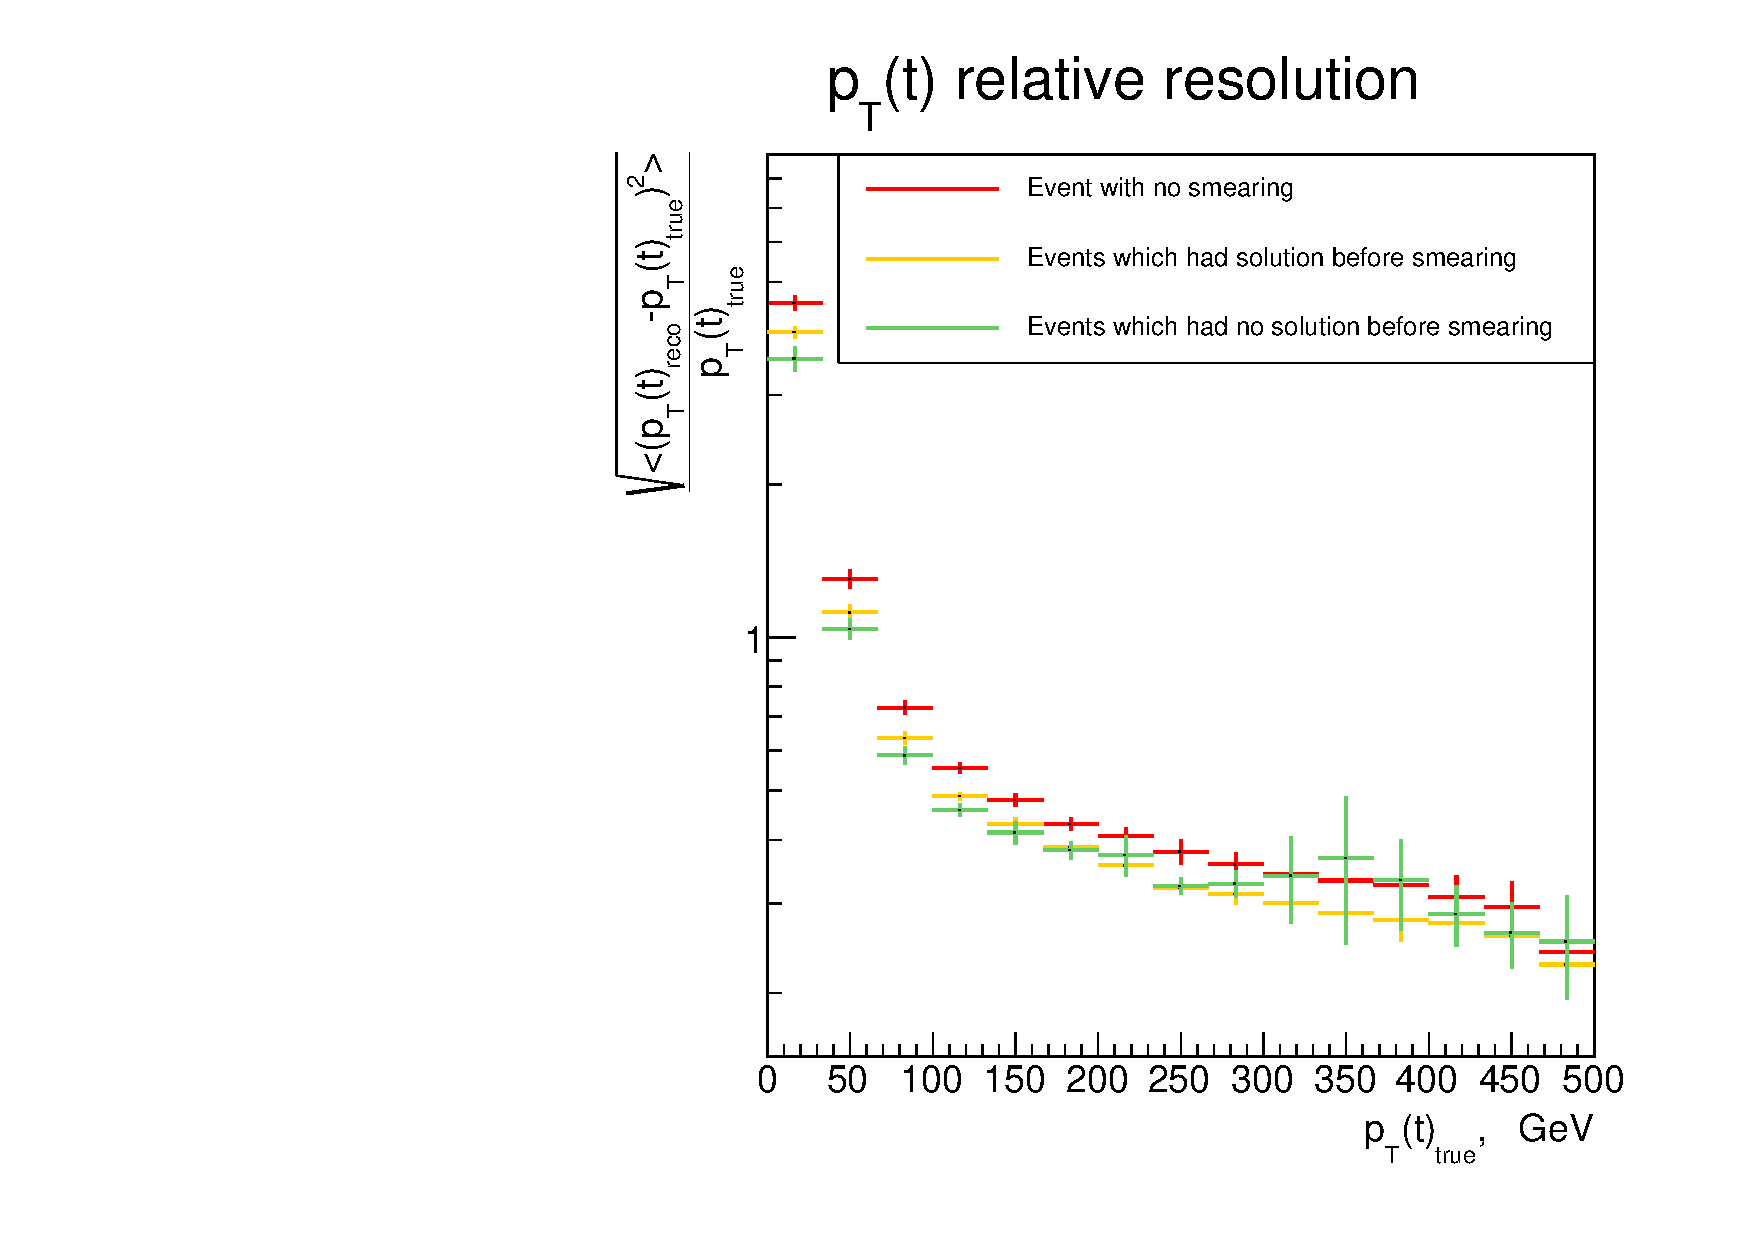
\includegraphics[width=0.8\textwidth]{/home/dolinska/Dropbox/desy_plots/Thesis/Jenya/10_appendices/KinReco/smearing-Motivation/RMS_pt.pdf}
  \caption{Relative resolution of the solutions which appear only due to smearing (green), smeared solutions which appear in the 
  event even without smearing (yellow) and solutions if no smearing is applied (red).}
  \label{fig:RMSsmear}
\end{figure}

% \begin{figure}[h]
%   \centering
% %   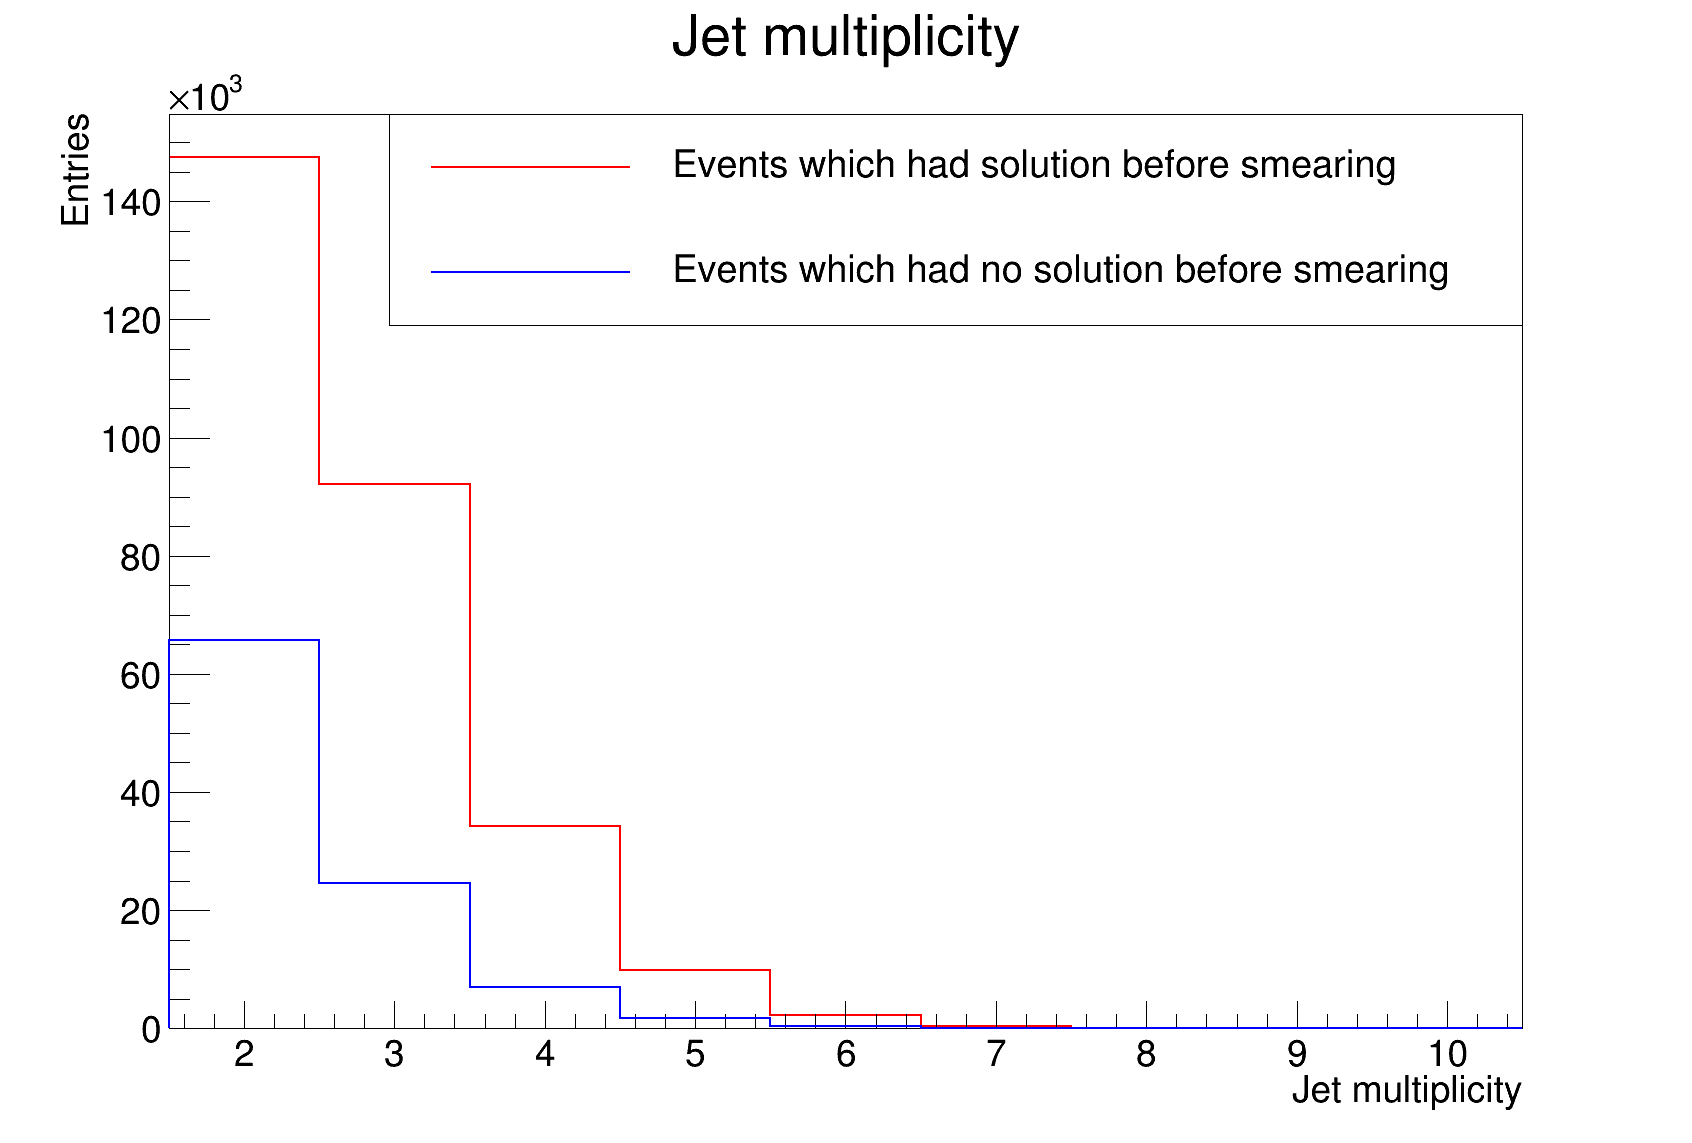
\includegraphics[width=1.0\textwidth]{10_appendices/smearing/Jet_Mult.png}
%   \caption{Jet multiplicity in the events where the solution of the kinematic equations appear only due to 
%   smearing (blue) and in the events where solutions were present before smearing (red).}
%   \label{fig:multSmear}
% \end{figure}